\documentclass[12pt]{article}
\usepackage[utf8]{inputenc}
\usepackage[T1]{fontenc}
\usepackage[spanish]{babel}
\usepackage{amsmath,amssymb,mathtools}
\usepackage{graphicx}
\usepackage{float}
\usepackage[margin=1in]{geometry}
\usepackage{parskip}
\usepackage{microtype}





\title{Dynamics of Public Health Expenditure in Peru: Evidence of Structural Breaks and Time-Series Analysis (1980–2022)}
\author{Luciano Díaz Tejada}
\date{Lima, July 2025}

\begin{document}
\maketitle
\section{Introduction}

Discussing public health expenditure in Peru means facing one of the country’s most complex paradoxes: although its importance is widely acknowledged, for decades it has been relegated in practice. Despite prolonged periods of economic growth since the 1990s, state investment in health has not kept pace. In 2022, for example, public health expenditure barely reached 3.91\% of GDP, well below the 6\% recommended by the Pan American Health Organization (Pan American Health Organization [PAHO], 2014). The COVID-19 pandemic merely laid bare that fragility: it showed how quickly hospitals collapse, how unequal infrastructure is, and how the lack of planning exacts a toll precisely when it is most needed.

This paper begins with a question many have asked, but which has rarely been addressed with rigorous tools: why, despite sustained economic growth, has Peru failed to consolidate an ambitious and stable public health policy? To answer it, I link economic history with statistical analysis. I apply ADF tests with dummy variables, log-linear models, and the Bai and Perron (2003) test to identify structural breaks in the expenditure series for 1980–2022. The results suggest three major phases: stagnation before 1992, strong expansion through 2009, and a more moderate growth stage thereafter. The hypothesis is clear: public health spending has not responded solely to technical or demographic criteria, but to shocks, fiscal constraints, and political decisions that have often been reactive. Looking closely at those moments—where spending accelerates, when it stalls, and why—helps to understand how we got here and what obstacles must be overcome to move forward.

\bigskip
\bigskip
\section{Literature Review}

\subsection{Crises, reforms, and the trajectory of spending}

The 1980s were a critical period for Peru. The state faced a devastating combination: debt crisis, hyperinflation, and political violence. In that context, maintaining a functional health system was simply unfeasible. Contreras and Cueto (2007) show how these crises reduced public health spending to minimal levels. The econometric analysis in this study supports that reading: prior to 1992, there is no significant upward trend in log spending, indicating institutional paralysis more than a deliberate budgetary decision.

The turning point comes in 1992. The structural reforms following hyperinflation, as described by Gonzales de Olarte (1998), marked a shift in the fiscal approach. A period of sustained growth in health spending begins—with an average rate of 11.4\% per year in logarithms—driven both by the recovery of fiscal revenues and by pent-up needs. This does not mean that the state prioritized health as a core policy, but it did mean there was fiscal room to maneuver. During this period there were advances: the Organisation for Economic Co-operation and Development (OECD, 2017) documents an expansion in coverage, although it warns that structural problems—such as institutional fragmentation—remained. Jaramillo and Parodi (2003) also highlight how rigid fiscal rules hindered ambitious planning. The econometric model shows that, without controlling for breaks, the residuals exhibit high volatility, suggesting that spending increases were more ad hoc responses than a state policy.

\subsection{Institutional fragmentation and limited capacity}

The structure of the health system is another major challenge. Mendoza-Arana et al. (2018) describe a dispersed institutional landscape: the Ministry of Health (MINSA), EsSalud, military health services, and subnational governments operate with limited coordination and without a clear lead authority. The OECD (2025), from an external perspective, confirms this: fragmentation limits both efficiency and the capacity to respond to crises, becoming a structural obstacle. This helps explain why, even as the budget increased between 1992 and 2009, the outcomes in effective coverage and equity were modest.

Between 2013 and 2022, EsSalud continued to show large gaps between regions, a shortage of medical personnel, and chronic infrastructure deficits. In addition, the study by Coaquira and Vilca (2023), which uses the Gini coefficient to measure inequality in provincial-level spending execution, highlights significant territorial disparities. This suggests that having more resources is not enough if there is no institutional capacity to execute them properly.

\subsection{Health crises and reactive responses}

Crises have been turning points, but rarely engines of deep reform. The 1991 cholera epidemic forced a reaction, as did the COVID-19 pandemic in 2020. In both cases there were spending spikes, but not sustained transformations (Mendoza-Arana et al., 2018). The multiple-breaks model detects another inflection in 2009, coinciding with the implementation of Universal Health Insurance and the H1N1 epidemic. From that point, the model incorporates an additional slope in the growth rate of spending. In other words, there is no deceleration but a moderate acceleration: an additional 3.3\% annual growth (in logs) is added to the rate prevailing since 1992. This raises total growth to approximately 14.7\% per year in logs from 2009 onward, signaling continuity rather than rupture.

ENSUSALUD data after 2009 show small improvements in perceived quality but also reflect that many structural shortcomings remain unresolved. The 6\% of GDP target for public health expenditure, proposed by PAHO (2014), remains just that: a pending target not yet achieved. Major health crises in Peru have functioned as catalysts for spending but rarely as points of institutional inflection. The 1991 cholera epidemic or the 2020 COVID-19 pandemic served to inject resources, but not to transform the system at its core (Mendoza-Arana et al., 2018).

\subsection{Public health and quantitative studies}

Public health, according to Winslow (1920), Acheson (1988), and the WHO (1998), is not limited to medical care; it is a collective commitment to prevention, well-being, and equity. Analyzing how it is financed reveals how much—and in what ways—a state prioritizes that well-being. In other countries, the topic has been addressed with econometric tools.

In China, Zheng et al. (2020) used ARIMA models to forecast the evolution of health expenditure. In Turkey, Atilgan et al. (2016) and Ilgun et al. (2023) analyzed how inflation, income, and reforms affect health spending. In Pakistan, Ullah et al. (2021) used a similar approach. In Peru, by contrast, there are few studies that combine statistical techniques with a long-term reading of health spending. This work seeks to fill that gap: by applying ADF tests with dummy variables, log-linear transformations, and multiple-break models, it identifies key moments in the spending trajectory and connects them to institutional changes. Understanding these cycles is crucial if we wish to avoid repeating past mistakes.

\bigskip
\bigskip
\bigskip
\bigskip
\bigskip
\bigskip
\bigskip
\bigskip
\bigskip
\bigskip
\bigskip
\bigskip
\bigskip
\bigskip
\section{Methodology}

Two fundamental problems arise in analyzing public health expenditure. First, before 1997, Peru’s health system was fragmented into three separate public subsystems: the Social Health Insurance administered by the then Peruvian Institute of Social Security (IPSS, now EsSalud); health services under the Ministry of Health (MINSA); and the health system for the Armed Forces and the National Police. This structure changed from 1997 onward, when these components began to be considered jointly within public health expenditure (Economic Commission for Latin America and the Caribbean [ECLAC] \& PAHO, 2013).

It is not possible—or at least extremely difficult—to access detailed data on IPSS expenditures prior to that date because of its institutional nature. The institute operated as an autonomous, decentralized agency with its own budget, outside the direct control of the Treasury. Its financing came mainly from a tripartite contribution scheme (workers, employers, and the state), which set it apart from the traditional budgeting frameworks of general government (ECLAC \& PAHO, 2013).

Moreover, until the mid-1990s, Peru’s public budget was organized by executing entity rather than by function. This structure makes it difficult to properly consolidate public spending in specific sectors such as health (Ministry of Economy and Finance [MEF], 2020). Only with the implementation of the Programmatic Functional Classification, introduced within the budget system reform in 1997, did execution by MINSA, EsSalud, and other entities begin to be systematically integrated under the category of “public health” (PAHO, 2008).

This was compounded by institutional weaknesses such as lack of transparency, limited oversight, and the absence of interoperable information systems, in a context where the Peruvian state had not yet advanced toward digitization nor adopted modern practices of fiscal management. Before National Health Accounts existed, fiscal statistics were fragmented, incomplete, and in many cases unaudited (PAHO, 2012).

This is why the decision was made to use only Central Government expenditure as the reference, given that this was the only sector for which information was available. For years after 1997, public health expenditure excluded social health insurance and payments to the police and military health services, as these were not recorded prior to 1997. In other words, only MINSA and regional expenditures were considered. However, this method does not materially alter the predictions of the constructed series, since health services spending since 1996 has been relatively stable (MINSA \& WHO, 2015). This can be seen in the close similarity between Figures 1 and 2.

The second problem lies in the different databases used to compile information. For 1980–1991, I relied on Portocarrero (1992), which systematizes accounting for state spending and includes state spending on health. For 1991–1995, I used Cruz (1998), which is also based on MINSA figures. Between 1995 and 2000, I used the National Health Accounts (MINSA, 2015). Finally, for 2000–2022, I used World Health Organization data (2025).

The choice of these databases was not arbitrary: given the scarcity of primary sources for the selected years, secondary sources were used for the cases prior to 1995. For the later period, World Health Organization data were preferred. This is because, on the one hand, out-of-pocket spending is not fully captured by MINSA, which leads to an overestimation of public spending when private spending is underestimated (as a share) (World Bank, 2016); on the other hand, “Peru’s health information system is not standardized across subsystems and it is difficult to link personal health data across entities. This hinders national measurement of activities, quality, or outcomes” (OECD, 2017).

While data prior to the 2000s may be underestimated precisely because they are not standardized, this does not prevent building a time series such as that shown in Figure 2.

\bigskip


\begin{figure}[H]
\centering{Figure 1: Total public health expenditure between 1996 and 2022 in thousands of 2007 soles}
\par\vspace{0.8em}
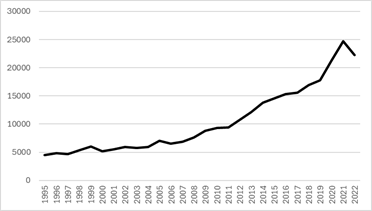
\includegraphics[width=0.5\linewidth]{Imagen2.png}

{\footnotesize Author’s elaboration. Information from WHO (2025) and MINSA (2012).}
\end{figure}



\begin{figure}[H]
\centering{Figure 2: Central Government expenditure between 1980 and 2022 in thousands of 2007 soles}
\par\vspace{0.8em}
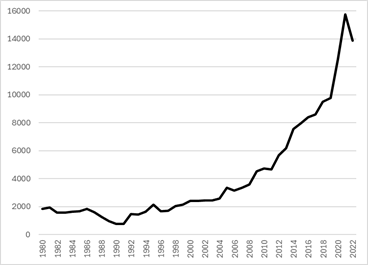
\includegraphics[width=0.5\linewidth]{Imagen3.png}

{\footnotesize Author’s elaboration. Information from WHO (2025) and MINSA (2012).}
\end{figure}

With the information clarified, it is possible to manipulate it in such a way as to offer answers about the processes behind health spending over the years. To reduce variance—and without loss of generality—the values in the table were log-linearized, yielding the following figure.

\bigskip
\bigskip
\bigskip

\begin{figure}[H]
\centering{Figure 3: Log-linearized Central Government expenditure between 1980 and 2022 in thousands of 2007 soles}
\par\vspace{0.8em}
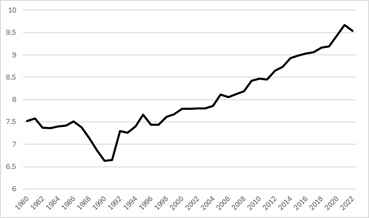
\includegraphics[width=0.5\linewidth]{Imagen4.png}

{\footnotesize Author’s elaboration. Information from Portocarrero (1992), Cruz (1998), MINSA (2012), and WHO (2025).}
\end{figure}

Since this is a time series, the functional form of health expenditure can be expressed as an autoregressive process. To estimate its optimal form, it is necessary to follow the procedure established by Box \& Jenkins (1976). Observing the series, a trend is clearly present. Thus, the first equation to be estimated would take the following form:

\begin{center}
\title{Equation 1: Functional form of Public Expenditure}
\end{center}
\begin{equation}
public\_expenditure_{t}= \beta + \gamma t + \sum_{i=1}^{p} \delta_{i}public\_expenditure_{t-i} + \alpha^{\top} X + \epsilon_{i}
\end{equation}

Correlation tests suggest the possible presence of a unit root, which is confirmed by applying the Augmented Dickey-Fuller (ADF) test; results are reported in Annex 3. Therefore, I use both the Zivot–Andrews test and the Bai–Perron test to render the series stationary. The results show three structural breaks: Zivot–Andrews identifies a break in 2004, while Bai–Perron detects breaks in 1992 and 2009. All three are significant (see Annexes 4 and 5). Subsequently, to analyze model seasonality, Fourier trigonometric functions were applied, following the methodology proposed by Seminario (2006), which allows more flexible control of seasonality. However, the results were not statistically significant (see Annex 6). That is, public health expenditure in Peru does not have a cyclical behavior.

To see whether these procedures help address the unit-root problem, I estimate the ADF regression in the following form:

\begin{center}
Equation 2: Augmented Dickey–Fuller test with a structural break (Zivot–Andrews)
\end{center}
\begin{equation}
\Delta public\_expenditure_{t} = \beta + \gamma t + \rho \, public\_expenditure_{t-1} + \sum_{i=1}^{p-1} \delta_{i} \, \Delta public\_expenditure_{t-i} + \theta_{1} D_{04} + \varepsilon_{i}
\end{equation}

\bigskip
\bigskip
\bigskip
\bigskip

\begin{center}
Where:
\end{center}
\begin{equation*}
D_{92}=1,\ \text{if } t>1992,\ \text{and } 0\ \text{otherwise}
\end{equation*}
\begin{equation*}
D_{09}=1,\ \text{if } t>2009,\ \text{and } 0\ \text{otherwise}
\end{equation*}

\bigskip
\begin{center}
Equation 3: Augmented Dickey–Fuller test with multiple structural breaks (Bai–Perron)
\end{center}
\begin{equation}
\small
\Delta public\_expenditure_{t} = \beta + \gamma t + \rho \, public\_expenditure_{t-1} + \sum_{i=1}^{p-1} \delta_{i} \, \Delta public\_expenditure_{t-i} + \theta_{1} D_{92} + \theta_{2} D_{09} + \varepsilon_{i}
\end{equation}
\begin{center}
Where:
\end{center}
\begin{equation*}
D_{92}=1,\ \text{if } t>1992,\ \text{and } 0\ \text{otherwise}
\end{equation*}
\begin{equation*}
D_{09}=1,\ \text{if } t>2009,\ \text{and } 0\ \text{otherwise}
\end{equation*}

Note that the number of lags in the summation is defined by the value that minimizes the Schwarz and Akaike criteria.

I then estimate the residual function. To verify whether the identified structural breaks are sufficient to guarantee stationarity of the model, I complement the analysis by applying the Hodrick–Prescott filter. This is important because it allows the decomposition of trend and cycle, making it possible to track moments associated with lower (negative) and higher (positive) health spending.

\section{Results}

As mentioned above, Annexes 4 and 5 present the structural-break results identified by the Zivot–Andrews and Bai–Perron tests, respectively. Since the two tests detect breaks at different moments, the question arises: which should be used? The one that, when included in the Augmented Dickey–Fuller test, renders the series stationary. The relevant tests are shown in Annexes 7 and 8. The Zivot–Andrews break in 2004 does not render the series stationary; the Bai–Perron results do. Hence, I focus on the latter. From this point forward, those results are used to transform the series.
The number of lags that minimizes the Schwarz and Akaike criteria is 0, so the equation to be estimated takes the following form:

\begin{center}
Equation 4: Augmented Dickey–Fuller test to be estimated
\end{center}
\begin{equation}
\Delta public\_expenditure=\beta+\gamma t+\rho public\_expenditure_{t-1}+\theta_1\ D_{92}+\theta_2\ D_{09}\ +\epsilon_i
\end{equation}

As noted earlier, results can be found in Annex 8. Interpreting the results, both 1992 and 2009 are decisive for the increase in public health expenditure. With this new information, and given that it is not necessary to difference the series to render it stationary, I evaluate a new equation as follows:

\bigskip
\bigskip
\begin{center}
Equation 5: Final equation to be estimated
\end{center}
\begin{equation}
public\_expenditure_t=\beta+\gamma t+\rho public\_expenditure_{t-1}+ \theta_1 D_{92}+\theta_2 D_{09} + \theta_3 DT_{92}+θ_4DT_{09}+ \epsilon_i
\end{equation}
\begin{center}
    Where:
\end{center}
\begin{equation*}
{DT}_{92}=t,\ \text{if } t>1992,\ \text{and } 0\ \text{otherwise}
\end{equation*}
\begin{equation*}
{DT}_{09}=t,\ \text{if } t>2009,\ \text{and } 0\ \text{otherwise}
\end{equation*}

Since the dummy corresponding to the 2009 break is not statistically significant, I conclude that the change observed in that year is reflected mainly in the slope of the series. Based on this, the final results are presented in Table 1.

The estimated econometric model provides a clearer understanding of how public health expenditure in Peru has changed in recent decades. One of the first elements to highlight is the inertia in the time series: the coefficient on the lagged expenditure (SERIES02(-1)), in logs, is 0.28. This means that if spending grows by 1\% in one year, the following year it tends to increase by an additional 0.28\% purely by carryover. However, the most interesting findings arise when analyzing the trend. Before 1992, spending followed a strongly negative slope: the trend coefficient (@TREND) is −0.067, equivalent to an average annual decline of 6.7\%. This supports what other studies have noted about the collapse of the state apparatus during the 1980s: a paralyzed health system with neither room nor capacity to respond.

\begin{figure}[H]
\centering{Table 1: Regression results}
\par\vspace{0.8em}

\includegraphics{Imagen5.png}
{\footnotesize Author’s elaboration.}
\end{figure}

In 1992, a significant change occurred. The model detects an immediate jump in the level of spending, represented by the dummy D92, whose coefficient of 0.399 is equivalent to an increase of almost 49\% in that year. However, the change is not limited to a one-off increase: from that moment on, the slope shifts completely. From 1992 onward, public health spending grows by an average of 11.4\% per year, as shown by the positive coefficient on TREND92 (0.108). This marks a structural break in the spending trajectory, in contrast with the declining trend observed in the prior years.

In 2009, the model detects another break: the slope changes again, this time with an additional coefficient of 0.0327. This implies that since 2009 the growth rate accelerates further: to the 11.4\% that had been in place since 1992, another 3.3\% per year is added. It is not a deceleration, but an intensification of growth. Thus, public health expenditure has followed a cumulative path, with two key points—1992 and 2009—that mark profound changes in its dynamics. These results are not just numbers: they help explain how and when the state began to invest more, and how well it has managed to sustain that effort.

Finally, is presented the error-correlation test using the Ljung–Box statistic, which shows that errors are not autocorrelated—implying that the disturbance term behaves as white noise.

\begin{figure}[H]
\centering{Table 2: Correlogram of Q-statistics}
\par\vspace{0.8em}
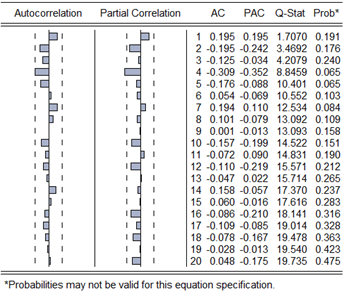
\includegraphics{Imagen6.png}

{\footnotesize Author’s elaboration.}
\end{figure}

\begin{figure}[H]
\centering{Figure 4: Evolution of residuals}
\par\vspace{0.8em}
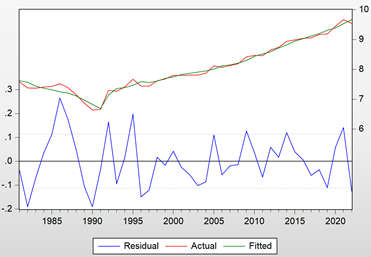
\includegraphics{Imagen7.png}

{\footnotesize Author’s elaboration.}
\end{figure}

Since the disturbance terms behave as white noise and the series has become stationary, 1992 and 2009 are key years in the time-series analysis. To analyze these results in greater detail, I applied a Hodrick–Prescott filter, obtaining the following:

\begin{figure}[H]
\centering{Figure 5: Hodrick–Prescott filter on the time series}
\par\vspace{0.8em}
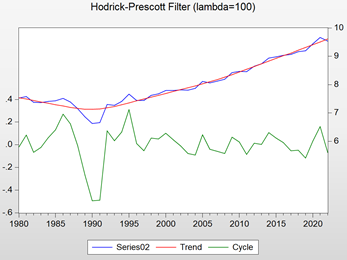
\includegraphics{Imagen8.png}

{\footnotesize Author’s elaboration.}
\end{figure}

This confirms that, until 1992, the spending trend was decreasing (−0.0671 on average), while thereafter it becomes positive. In 2009, the trend “increases further,” which the above model explains through the slope break in that year. In sum, the dynamic analysis of real public expenditure in Peru reveals three clearly differentiated stages. Before 1992, the trend was negative, equivalent to an annual decline of approximately 6.48\% in the absence of structural reforms. This pattern reverses from 1992, with an immediate increase in the spending level of about 49.0\% and a positive change in the growth slope of approximately 11.4\% per year. From 2009, there is a new structural inflection, with an additional acceleration of about 3.3\% per year. These estimates suggest that spending performance has been heavily conditioned by institutional breaks that redefined both its level and its long-run pace of expansion.

How do these events relate to the cases mentioned earlier? The empirical results not only confirm what authors such as Contreras and Cueto (2007) warned about the fiscal collapse of the 1980s; they also help specify how and when the pattern of health investment was reconfigured. The nearly 49\% jump in 1992 and the slope break that accelerates spending by 11.4\% annually reflect, in numerical terms, what Gonzales de Olarte (1998) described as the shift toward a model of fiscal discipline and expenditure reordering. The 1992–2009 period—identified by studies such as Alvarado et al. (2007) and Jaramillo and Parodi (2003) as a phase of expansion with bottlenecks—appears here as a phase of intense but constrained recovery, where spending growth did not always translate into structural improvements.

The second break, in 2009, adds a further positive slope of 3.3\% per year, aligning with reforms such as Universal Health Insurance and shocks such as the H1N1 pandemic, reinforcing the view of Mendoza-Arana et al. (2018) and the OECD (2025) about the state’s reactive logic in the face of health emergencies. In other words, the spending trajectory has not been random: it has responded to historical events and been shaped by institutional architecture and the fiscal decisions of the moment. It is also worth noting that health spending does not exhibit cyclical behavior, so it is largely explained by these breaks (which also explains the large $R^2$).

While the model shows significant cumulative growth, this should not be read with excessive optimism. Spending has increased, yes, but it does so from a very low base, and even in 2022 it does not exceed 4\% of GDP. PAHO (2014) sets a minimum threshold of 6\% of GDP to ensure a functional public health system, and Peru remains far from that target. The persistence of a low GDP share allocated to the sector reveals that, despite absolute increases, structural constraints persist: institutional fragmentation, low execution capacity, and a spending model that reacts to crises but does not sustain itself. In this sense, the identified breaks are both evidence of adaptation and a reminder of a persistent weakness: public health in Peru still does not occupy the place it should in the state’s hierarchy of priorities.

\section{Conclusions}

Over the last four decades, public health expenditure in Peru has followed a trajectory marked more by ups and downs than by a consistent public policy. The econometric analysis confirms what many studies have warned from historical, institutional, or fiscal perspectives: there has been no sustained logic of expansion, but rather moments of rupture, almost always induced by economic or health crises.

Until 1992, spending remained practically stagnant, reflecting the deterioration of the state apparatus during the years of hyperinflation, political violence, and institutional collapse. From that year, there is a significant shift. Spending begins to grow, but it does so from very low levels, as a response to macroeconomic stabilization rather than a structural transformation of the public health system. Then, in 2009, the pattern changes again, with additional acceleration of spending. This new phase coincides with the implementation of Universal Health Insurance and the fallout from another health emergency, but it was not accompanied by deep reforms either. The model shows clearly that spending increases have been closely tied to moments of tension or external pressure. There is no evidence of a long-term plan or a sustained strategy to strengthen the health system. Even when spending increased, the persistent level below 6\% of GDP—the minimum recommended by international organizations—reveals that improvements have been more reactive than structural.

In short, public health expenditure in Peru has not followed a technical logic guided by the system’s real needs, but has been conditioned by political conjuncture, social pressure, and institutional constraints. Unless these root causes are addressed, the observed pattern may repeat itself: temporary increases in response to crises, followed by new stages of stagnation. Breaking this cycle requires more than larger budgets: it demands rethinking the state’s role in public health, strengthening institutional capacity, and treating health as a strategic public good on a sustained basis.

\section{References}

Acheson, D. (1988). On the state of public health. Public Health, 102(5):431–437. doi: .

Atilgan, E., Kilic, D., \& Ertugrul, H. M. (2017). The dynamic relationship between health expenditure and economic growth: Is the health-led growth hypothesis valid for Turkey? \textit{The European Journal of Health Economics}, 18(5), 567–574. https://doi.org/10.1007/s10198-016-0810-5

Bai, J., \& Perron, P. (2003). Critical values for multiple structural change tests. \textit{The Econometrics Journal}, 6(1), 72–78. http://www.jstor.org/stable/23113649

Box, G.E.P. \& Jenkins, G.M. (1976). \textit{Time Series Analysis: Forecasting and Control}. Holden Day.

Coaquira Vargas, M. V., \& Vilca Colquehuanca, G. L. (2023). Effect of public health expenditure on poverty in the provinces of Peru. \textit{Revista Científica de la UCSA}, 10(3), 80–94.

Economic Commission for Latin America and the Caribbean [ECLAC] \& Pan American Health Organization [PAHO]. (2013). \textit{Social protection systems in Latin America and the Caribbean: Peru}. Santiago: United Nations. https://hdl.handle.net/11362/40365

Economic Commission for Latin America and the Caribbean [ECLAC]. (2010). \textit{Fiscal institutions in Latin America}. Santiago: United Nations. https://hdl.handle.net/11362/3402

Contreras, C., \& Cueto, M. (2007). \textit{Historia del Perú Contemporáneo: Desde las luchas por la independencia hasta el presente} (4th ed.). Instituto de Estudios Peruanos (IEP).

Cruz, M. (1998). Health expenditure. \textit{Revista de la Facultad de Ciencias Económicas}. Universidad Nacional Mayor de San Marcos.

Gonzales de Olarte, E. (1998). \textit{El neoliberalismo a la peruana: Economía política del ajuste estructural, 1990–1995}. Instituto de Estudios Peruanos (IEP); Consorcio de Investigación Económica. http://documents.worldbank.org/curated/en/441041481748303633

İlgün, G., Konca, M., \& Sönmez, S. (2023). The relationship between the Health Transformation Program and health expenditures: Evidence from an autoregressive distributed lag testing approach. \textit{Value in Health Regional Issues}, 38, 101–108. https://doi.org/10.1016/j.vhri.2023.08.003

Jaramillo, M., \& Parodi, S. (2004). \textit{El Seguro Escolar Gratuito y el Seguro Materno Infantil: Análisis de su incidencia e impacto sobre el acceso a los servicios de salud y sobre la equidad en el acceso}. GRADE.

Mendoza-Arana, P. J., Rivera-Del Río, G., Gutiérrez-Villafuerte, C., \& Sanabria-Montañez, C. (2018). The health sector reform process in Peru. \textit{Revista Panamericana de Salud Pública}, 42, e74.

Ministry of Economy and Finance [MEF]. (2020). \textit{Manual of Budget Classifications of the Public Sector}. Dirección General de Presupuesto Público.

Ministry of Health [MINSA] \& World Health Organization [WHO]. (2015). \textit{National Health Accounts: Peru 1995–2012}.

World Health Organization. (1998). \textit{Health Promotion. Glossary}.

Pan American Health Organization [PAHO]. (2008). \textit{Public health expenditure in Latin America and the Caribbean: Trends and challenges}. Washington, D.C.: PAHO. https://iris.paho.org/handle/10665.2/3128

Pan American Health Organization [PAHO]. (2012). \textit{Health systems in Latin America and the Caribbean: Foundations, evolution and challenges}. https://iris.paho.org/

Pan American Health Organization [PAHO]. (2014). \textit{Strategy for Universal Access to Health and Universal Health Coverage} (Official Document 53/5, Rev. 2).

Organisation for Economic Co-operation and Development [OECD]. (2025). \textit{OECD Reviews of Health Systems: Peru 2025}. OECD Publishing.

Organisation for Economic Co-operation and Development [OECD]. (2017). \textit{OECD Reviews of Health Systems: Peru 2017}. OECD Publishing.

Portocarrero, F. (1993). \textit{El gasto público en salud, Perú: 1980–1992}. Informe de coyuntura. Evolución de la Economía Peruana.

Seminario, B. (2006). Economic growth in Peru: 1950–2004. Reforms and structural continuity. \textit{Revista de Estudios Económicos}, (13), 9–62. Central Reserve Bank of Peru.

Ullah, I., Ullah, A., Ali, S., Poulova, P., Akbar, A., Haroon Shah, M., Rehman, A., Zeeshan, M., \& Afridi, F. E. A. (2021). Public Health Expenditures and Health Outcomes in Pakistan: Evidence from Quantile Autoregressive Distributed Lag Model. \textit{Risk Management and Healthcare Policy}, 14, 3893–3909. https://doi.org/10.2147/RMHP.S316844

Vermeersch, C. M. J. (2016). \textit{Health financing in Peru: Analysis of the current situation and policy challenges 2021}. World Bank Group.

Winslow, C. (1920). The Untilled Fields of Public Health. \textit{Science}, 51, 23–33. DOI:3

Zheng, A., Fang, Q., Zhu, Y., Jiang, C., Jin, F., \& Wang, X. (2020). An application of ARIMA model for predicting total health expenditure in China from 1978–2022. \textit{Journal of Global Health}, 10(1), 010803. https://doi.org/10.7189/jogh.10.010803

\section{Annexes}

\begin{figure}[H]
\centering{1. Public health expenditure between 1996 and 2022 (including EsSalud and services for the military and National Police)}
\par\vspace{0.8em}

\includegraphics[width=0.4\linewidth]{Imagen9.png}

{\footnotesize Author’s elaboration. Information from WHO (2025) and MINSA (2012).}
\end{figure}

\begin{figure}[H]
\centering{2. Central Government health expenditure between 1980 and 2022 (excluding National Police and social insurance outlays)}
\par\vspace{0.8em}

\includegraphics[width=0.6\linewidth]{Imagen10.png}

{\footnotesize Author’s elaboration. Information from Portocarrero (1992), Cruz (1998), MINSA (2012), and WHO (2025).}
\end{figure}

\begin{figure}[H]
\centering{3. Results of the Augmented Dickey–Fuller test}
\par\vspace{0.8em}

\includegraphics{Imagen11.png}

{\footnotesize Author’s elaboration.}
\end{figure}

\begin{figure}[H]
\centering{4. Zivot–Andrews test to determine the optimal number of roots}
\par\vspace{0.8em}
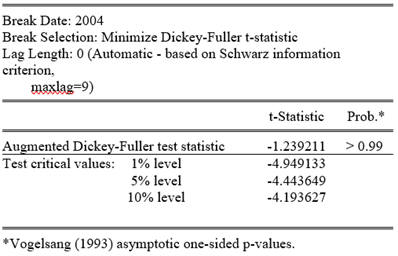
\includegraphics{Imagen12.png}

{\footnotesize Author’s elaboration.}
\end{figure}

\begin{figure}[H]
\centering{5. Bai–Perron test to determine the optimal number of roots}
\par\vspace{0.8em}

\includegraphics{Imagen13.png}

{\footnotesize Author’s elaboration.}
\end{figure}

\begin{figure}[H]
\centering{6. Results of Fourier trigonometric approximation}
\par\vspace{0.8em}

\includegraphics{Imagen14.png}

{\footnotesize Author’s elaboration. Note that the following functional form was used:
$y_t=\alpha+\beta t+\rho y_{t-1}+\delta\cdot\sin\!\left(\frac{2\pi t}{5}\right)+\theta\cdot\cos\!\left(\frac{2\pi t}{5}\right)+\epsilon_t$. The aim was to capture seasonality every 5 years, aligning with presidential elections. Even when testing 2-, 3-, or 4-year seasonality, the result is not significant. For details, see Seminario (2006).}
\end{figure}

\begin{figure}[H]
\centering{7. Results of including Zivot–Andrews structural breaks as regressors in the ADF}
\par\vspace{0.8em}

\includegraphics{Imagen15.png}

{\footnotesize Author’s elaboration. Note that the coefficient on SERIES02(-1), the first lag of public spending, is not significant. That is, the series does not become stationary. No explanatory lags are used because this choice minimizes the Schwarz and Akaike criteria. Both the Zivot–Andrews and Bai–Perron tests found the system’s trend and the slope-change dummies (trend breaks) to be non-significant, so they were excluded.}
\end{figure}

\begin{figure}[H]
\centering{8. Results of including Bai–Perron structural breaks as regressors in the ADF}
\par\vspace{0.8em}

\includegraphics{Imagen16.png}

{\footnotesize Author’s elaboration.}
\end{figure}


\end{document}